\documentclass{report}

\usepackage[T1]{fontenc}
\usepackage[polish]{babel}
\usepackage[utf8]{inputenc}
\usepackage{lmodern}
\usepackage{longtable}
\usepackage{multirow}
\usepackage{enumerate}
\usepackage{array}
\newcolumntype{C}[1]{>{\centering\let\newline}}
\selectlanguage{polish}
\usepackage{xcolor}
\usepackage[colorlinks]{hyperref}
\usepackage[anythingbreaks]{breakurl}
\usepackage{textcomp}
\usepackage{listings}
\usepackage{color}
\definecolor{pblue}{rgb}{0.13,0.13,1}
\definecolor{pgreen}{rgb}{0,0.5,0}
\definecolor{pred}{rgb}{0.9,0,0}
\definecolor{pgrey}{rgb}{0.46,0.45,0.48}

\usepackage{listings}
\lstset{language=Java,
  showspaces=false,
  showtabs=false,
  breaklines=true,
  showstringspaces=false,
  breakatwhitespace=true,
  commentstyle=\color{pgreen},
  keywordstyle=\color{pblue},
  stringstyle=\color{pred},
  basicstyle=\ttfamily,
  moredelim=[il][\textcolor{pgrey}]
  moredelim=[is][\textcolor{pgrey}]{\%\%}{\%\%}
}
\usepackage{graphicx}
\title{Dokumentacja projektu "Booka"}
\author{Miłosz Białczak (218295)\\ Mateusz Gniewkowski (218138)\\ Beata Szeląg (218139)}
\date{\today}

\begin{document}

\setlength{\LTleft}{-20cm plus -1fill}
\setlength{\LTright}{\LTleft}
\maketitle
\tableofcontents{}



\chapter{Wstęp}

	
	Celem projektu jest zaproponowanie, zaprojektowanie, implementacja i udokumentowanie systemu opartego o technologię Java EE. System jaki zamierzamy stworzyć ma umożliwić zarządzanie domową biblioteczką przeciętnemu użytkownikowi komputera. System powinien przede wszystkim dawać możliwość katalogowania i kategoryzowania książek z dowolnego punktu dostępowego. Wskazane jest więc użycie technologii pozwalających na stworzenie aplikacji webowej, które to wybraliśmy na podstawie analizy postawionych przez nas wymagań. Projekt obejmuje więc:
	\begin{enumerate}
		\item
		określenie celów
		\item
		pomysł realizacji postawionych celów
		\item
		analizę wymagań
		\item
		wybór technologii
		\item
		zaprojektowanie systemu		
		\item
		implementację systemu 	
		\item
		dokumentację techniczną (w postaci niniejszego dokumentu)
	\end{enumerate}	

	
	\section{Uzasadnienie biznesowe}
	
	Wraz ze wzrostem liczby książek coraz większą trudność sprawia utrzymanie ich w porządku, zwłaszcza jeżeli część książek została pożyczona od kogoś lub komuś - stąd pomysł na naszą aplikację. Nasza aplikacja (dalej zwana "Booką") ma umożliwić wygodne zarządzanie księgozbiorem. Daje ona możliwość zaznaczenia kto daną książkę pożyczył i kiedy powinien ją oddać oraz wiele innych przydatnych funkcjonalności, które zostaną opisane dogłębniej w niniejszym dokumencie.

\chapter{Analiza systemu}
	\section{Opis działania systemu}
	
	Systemem, który stworzono jest prosta aplikacja internetowa. Po uruchomieniu przeglądarki i wpisaniu odpowiedniego adresu użytkownikowi powinna pokazać się
	strona umożliwiająca zalogowanie się, lub rejestrację do systemu. Po zalogowaniu, strona przenosi użytkownika do strony głównej, z której użytkownik ma dostęp do swojego księgozbioru (rozumie się przez to możliwość dodawania, usuwania książek, jak i przeglądania go), do podglądu swoich znajomych, podglądania książek im i od nich pożyczonych, chatu, widoku umożliwiającego przeszukiwanie okolicznych bibliotek i do swojego konta Google (po uprzednim zalogowaniu się do niego), umożliwiającego przechowywania elektronicznych wersji książek w chmurze.
	
	\section{Wymagania funkcjonalne}
	
	
	%\begin{longtable}{|c|p{12cm}|}
	%\caption{Wymaganie funkcjonalne F\_XX} \label{tab:F_XX} \\ \hline
	%\multicolumn{2}{ |c| }{Nazwa wymagania} \\ \hline
	%ID & F\_XX \\ \hline
	%Opis & 	opis \\ \hline
	%Priorytet & wymagane/oczekiwane/opcjonalne \\ \hline
	%Powiązania & login/-  \\ \hline
	%\end{longtable} 
	
	
	
	
	\begin{longtable}{|c|p{12cm}|}
	\caption{Wymaganie funkcjonalne F\_00} \label{tab:F_00} \\ \hline
	\multicolumn{2}{ |c| }{Utworzenie konta} \\ \hline
	ID & F\_00 \\ \hline
	Opis & Użytkownicy nieposiadający kont mają możliwość ich założenia. Po wybraniu odpowiedniej opcji, na podany adres mailowy zostaje wysłana wiadomość zawierająca link potwierdzający rejestrację.  \\ \hline
	Priorytet & wymagane\\ \hline
	Powiązania & - \\ \hline
	\end{longtable} 
	
	
	\begin{longtable}{|c|p{12cm}|}
	\caption{Wymaganie funkcjonalne F\_01} \label{tab:F_01} \\ \hline
	\multicolumn{2}{ |c| }{Logowanie} \\ \hline
	ID & F\_01 \\ \hline
	Opis & 	Użytkownik posiadający konto może zalogować się do systemu\\ \hline
	Priorytet & wymagane\\ \hline
	Powiązania & - \\ \hline
	\end{longtable} 
	
	
	\begin{longtable}{|c|p{12cm}|}
	\caption{Wymaganie funkcjonalne F\_02} \label{tab:F_02} \\ \hline
	\multicolumn{2}{ |c| }{Wylogowanie} \\ \hline
	ID & F\_02 \\ \hline
	Opis & Zalogowany użytkownik może się wylogować \\ \hline
	Priorytet & wymagane\\ \hline
	Powiązania & - \\ \hline
	\end{longtable}
	
	\begin{longtable}{|c|p{12cm}|}
	\caption{Wymaganie funkcjonalne F\_03} \label{tab:F_03} \\ \hline
	\multicolumn{2}{ |c| }{Konfiguracja} \\ \hline
	ID & F\_03 \\ \hline
	Opis & 	Użytkownik ma możliwość konfiguracji swojego konta, a w szczególności ustawienia i zmiany hasła \\ \hline
	Priorytet & wymagane\\ \hline
	Powiązania & - \\ \hline
	\end{longtable} 
	
	
	
	\begin{longtable}{|c|p{12cm}|}
	\caption{Wymaganie funkcjonalne F\_04} \label{tab:F_04} \\ \hline
	\multicolumn{2}{ |c| }{Dodawanie pozycji do księgozbioru} \\ \hline
	ID & F\_04 \\ \hline
	Opis & 	Użytkownik może dodać nową pozycję do swojego księgozbioru. Powinien on określić jej tytuł, autora i kategorię. Jeżeli użytkownik posiada elektroniczną kopię książki na dysku lokalnym, lub obsługiwanym dysku sieciowym (serwer FPT), może ją zaimportować automatycznie. Jest możliwe importowanie całych katalogów naraz - aplikacja powinna reagować na zmiany w danym katalogu i automatycznie importować ich zawartość. \\ \hline
	Priorytet & wymagane \\ \hline
	Powiązania & -  \\ \hline
	\end{longtable} 
	
	\begin{longtable}{|c|p{12cm}|}
	\caption{Wymaganie funkcjonalne F\_05} \label{tab:F_05} \\ \hline
	\multicolumn{2}{ |c| }{Usuwanie pozycji z księgozbioru} \\ \hline
	ID & F\_05 \\ \hline
	Opis & 	Użytkownik może usunąć dowolną pozycję ze swojego księgozbioru. \\ \hline
	Priorytet & wymagane\\ \hline
	Powiązania & -  \\ \hline
	\end{longtable}
	
	\begin{longtable}{|c|p{12cm}|}
	\caption{Wymaganie funkcjonalne F\_06} \label{tab:F_06} \\ \hline
	\multicolumn{2}{ |c| }{Podgląd księgozbioru} \\ \hline
	ID & F\_06 \\ \hline
	Opis & 	Użytkownik może przeglądać swój księgozbiór. \\ \hline
	Priorytet & wymagane \\ \hline
	Powiązania & -  \\ \hline
	\end{longtable} 
	
	\begin{longtable}{|c|p{12cm}|}
	\caption{Wymaganie funkcjonalne F\_07} \label{tab:F_07} \\ \hline
	\multicolumn{2}{ |c| }{Przeszukiwanie księgozbioru} \\ \hline
	ID & F\_07 \\ \hline
	Opis & Użytkownik może przeszukiwać swój księgozbiór po nazwie, autorze, kategorii itp.\\ \hline
	Priorytet & wymagane \\ \hline
	Powiązania & F\_06  \\ \hline
	\end{longtable} 
	
	\begin{longtable}{|c|p{12cm}|}
	\caption{Wymaganie funkcjonalne F\_08} \label{tab:F_08} \\ \hline
	\multicolumn{2}{ |c| }{Przeszukiwanie zasobów bibliotecznych} \\ \hline
	ID & F\_08 \\ \hline
	Opis & Użytkownik powinien mieć możliwość przeglądania zasobów bibliotek miejskich. \\ \hline
	Priorytet & wymagane \\ \hline
	Powiązania & -  \\ \hline
	\end{longtable}
	
	\begin{longtable}{|c|p{12cm}|}
	\caption{Wymaganie funkcjonalne F\_09} \label{tab:F_09} \\ \hline
	\multicolumn{2}{ |c| }{Przeszukiwanie sklepów internetowych} \\ \hline
	ID & F\_09 \\ \hline
	Opis & Użytkownik powinien mieć możliwość wyszukiwania książek w zdefiniowanych sklepach \\ \hline
	Priorytet & oczekiwane  \\ \hline
	Powiązania & -  \\ \hline
	\end{longtable}
	
	\begin{longtable}{|c|p{12cm}|}
	\caption{Wymaganie funkcjonalne F\_10} \label{tab:F_10} \\ \hline
	\multicolumn{2}{ |c| }{Pożyczanie książek} \\ \hline
	ID & F\_10 \\ \hline
	Opis & Użytkownik powinien mieć możliwość oznaczenia książki jako pożyczonej (z uwzględnieniem komu owa książka została pożyczona). Informacja o pożyczonych komuś i od kogoś książkach powinna być dostępna w widoku księgozbioru.\\ \hline
	Priorytet & wymagane \\ \hline
	Powiązania & F\_06, F\_11   \\ \hline
	\end{longtable} 
	
	\begin{longtable}{|c|p{12cm}|}
	\caption{Wymaganie funkcjonalne F\_11} \label{tab:F_11} \\ \hline
	\multicolumn{2}{ |c| }{Oddawanie książek} \\ \hline
	ID & F\_11 \\ \hline
	Opis & System powinien dawać możliwość oddawania książek. \\ \hline
	Priorytet & wymagane \\ \hline
	Powiązania & F\_06, F\_10  \\ \hline
	\end{longtable}
	
	\begin{longtable}{|c|p{12cm}|}
	\caption{Wymaganie funkcjonalne F\_12} \label{tab:F_12} \\ \hline
	\multicolumn{2}{ |c| }{System notyfikacji} \\ \hline
	ID & F\_12 \\ \hline
	Opis & System powinien automatycznie informować użytkownika o akcjach z nim związanych (np. informacja o zbliżającym się terminie oddania książki). Notyfikacje powinny być możliwe do modyfikacji i wyłączenia.  \\ \hline
	Priorytet & oczekiwane \\ \hline
	Powiązania & -  \\ \hline
	\end{longtable}
	
	\begin{longtable}{|c|p{12cm}|}
	\caption{Wymaganie funkcjonalne F\_13} \label{tab:F_13} \\ \hline
	\multicolumn{2}{ |c| }{Dostęp do pozycji w wersjach elektronicznych} \\ \hline
	ID & F\_13 \\ \hline
	Opis & Jeżeli książka jest dostępna w wersji elektronicznej, powinno być możliwe otworzenie jej z poziomu aplikacji. \\ \hline
	Priorytet & oczekiwane \\ \hline
	Powiązania & -  \\ \hline
	\end{longtable} 
	
	
	\begin{longtable}{|c|p{12cm}|}
	\caption{Wymaganie funkcjonalne F\_14} \label{tab:F_14} \\ \hline
	\multicolumn{2}{ |c| }{Udostępnianie księgozbioru} \\ \hline
	ID & F\_14 \\ \hline
	Opis & Użytkownik powinien mieć możliwość udostępnienia swojego księgozbioru do podglądu innym użytkownikom (niekoniecznie z opcją czytania książek w wersji elektronicznej) \\ \hline
	Priorytet & opcjonalne \\ \hline
	Powiązania & -  \\ \hline
	\end{longtable} 
	
	\begin{longtable}{|c|p{12cm}|}
	\caption{Wymaganie funkcjonalne F\_15} \label{tab:F_15} \\ \hline
	\multicolumn{2}{ |c| }{Wysyłanie powiadomień do innych użytkowników} \\ \hline
	ID & F\_15 \\ \hline
	Opis & Użytkownik powinien mieć możliwość wysyłania powiadomień innym użytkownikom. Powiadomienia mogą dotyczyć próśb o pożyczenie, oddanie książki, udostępnienie podglądu księgozbioru itp. Powiadomienia mogą być wysyłane poprzez Facebooka, e-maila, lub aplikację. \\ \hline
	Priorytet & oczekiwane \\ \hline
	Powiązania & -  \\ \hline
	\end{longtable}
	
	
	
	\section{Wymagania niefunkcjonalne}
	
	%\begin{longtable}{|c|p{12cm}|}
	%\caption{Wymaganie niefunkcjonalne N\_XX} \label{tab:N_XX} \\ \hline
	%\multicolumn{2}{ |c| }{Nazwa wymagania} \\ \hline
	%ID & N\_XX \\ \hline
	%Opis & opis \\ \hline
	%Priorytet & wymagane/oczekiwane/opcjonalne \\ \hline
	%Powiązania & login/- \\ \hline
	%\end{longtable}
	
	\begin{longtable}{|c|p{12cm}|}
	\caption{Wymaganie niefunkcjonalne N\_00} \label{tab:N_00} \\ \hline
	\multicolumn{2}{ |c| }{Interfejs użytkownika} \\ \hline
	ID & N\_00 \\ \hline
	Opis & Aplikacja powinna posiadać ładny i przejrzysty graficzny interfejs użytkownika, możliwe intuicyjny i łatwy w obsłudze. \\ \hline
	Priorytet & oczekiwane \\ \hline
	Powiązania & - \\ \hline
	\end{longtable} 
	
	
	\begin{longtable}{|c|p{12cm}|}
	\caption{Wymaganie niefunkcjonalne N\_01} \label{tab:N_01} \\ \hline
	\multicolumn{2}{ |c| }{Odporność na utratę danych} \\ \hline
	ID & N\_01 \\ \hline
	Opis & Stworzenie mechanizmów w systemie odpowiedzialnych za cykliczną
	archiwizację stanu bazy danych oraz możliwość wczytania jej z pliku. \\ \hline
	Priorytet & oczekiwane \\ \hline
	Powiązania & - \\ \hline
	\end{longtable}
	
	\begin{longtable}{|c|p{12cm}|}
	\caption{Wymaganie niefunkcjonalne N\_02} \label{tab:N_02} \\ \hline
	\multicolumn{2}{ |c| }{Skalowalność} \\ \hline
	ID & N\_02 \\ \hline
	Opis & System powinien zapewnić możliwość jego rozbudowy pod względem rozmiaru \\ \hline
	Priorytet & oczekiwane \\ \hline
	Powiązania & - \\ \hline
	\end{longtable}
	
	\begin{longtable}{|c|p{12cm}|}
	\caption{Wymaganie niefunkcjonalne N\_03} \label{tab:N_03} \\ \hline
	\multicolumn{2}{ |c| }{Bezpieczeństwo danych} \\ \hline
	ID & N\_03 \\ \hline
	Opis & System powinien dbać o zapewnienie ograniczonego
	dostępu do przechowywanych informacji. \\ \hline
	Priorytet & wymagane \\ \hline
	Powiązania & - \\ \hline
	\end{longtable}
	
	\begin{longtable}{|c|p{12cm}|}
	\caption{Wymaganie niefunkcjonalne N\_04} \label{tab:N_04} \\ \hline
	\multicolumn{2}{ |c| }{Wydajność} \\ \hline
	ID & N\_04 \\ \hline
	Opis & System powinien reagować na zapytania użytkownika z opóźnieniem nie większym niż pół sekundy. \\ \hline
	Priorytet & oczekiwane \\ \hline
	Powiązania & - \\ \hline
	\end{longtable}
	
	
	\begin{longtable}{|c|p{12cm}|}
	\caption{Wymaganie niefunkcjonalne N\_05} \label{tab:N_05} \\ \hline
	\multicolumn{2}{ |c| }{Możliwość rozwoju} \\ \hline
	ID & N\_05 \\ \hline
	Opis & System powinien być zaplanowany w ten sposób, aby umożliwić dołączanie nowych funkcjonalności. \\ \hline
	Priorytet & oczekiwane \\ \hline
	Powiązania & - \\ \hline
	\end{longtable}


	\section{Wymagania technologiczne}
	
	
	%\begin{longtable}{|c|p{12cm}|}
	%\caption{Wymaganie technologiczne T\_XX} \label{tab:T_XX} \\ \hline
	%\multicolumn{2}{ |c| }{Nazwa wymagania} \\ \hline
	%ID & T\_XX \\ \hline
	%Opis & opis \\ \hline
	%Priorytet & wymagane/oczekiwane/opcjonalne \\ \hline
	%Powiązania & login/- \\ \hline
	%\end{longtable} 
	
	
	
	\begin{longtable}{|c|p{12cm}|}
	\caption{Wymaganie technologiczne T\_00} \label{tab:T_00} \\ \hline
	\multicolumn{2}{ |c| }{Java} \\ \hline
	ID & T\_00 \\ \hline
	Opis & Aplikacja powinna być stworzona w języku Java, wersja 8 lub wyższa. \\ \hline
	Priorytet & wymagane \\ \hline
	Powiązania & - \\ \hline
	\end{longtable} 
	
	
	\begin{longtable}{|c|p{12cm}|}
	\caption{Wymaganie technologiczne T\_01} \label{tab:T_01} \\ \hline
	\multicolumn{2}{ |c| }{SpringBoot} \\ \hline
	ID & T\_01 \\ \hline
	Opis & Serwer aplikacji powinien być napisany z wykorzystaniem framework'a Spring Boot. \\ \hline
	Priorytet & wymagane\\ \hline
	Powiązania & - \\ \hline
	\end{longtable} 
	
	
	\begin{longtable}{|c|p{12cm}|}
	\caption{Wymaganie technologiczne T\_02} \label{tab:T_02} \\ \hline
	\multicolumn{2}{ |c| }{MySQL} \\ \hline
	ID & T\_02 \\ \hline
	Opis & Wykorzystywanym systemem bazodanowym powinien być MySQL. \\ \hline
	Priorytet & wymagane \\ \hline
	Powiązania & - \\ \hline
	\end{longtable}
	
	
	\begin{longtable}{|c|p{12cm}|}
	\caption{Wymaganie technologiczne T\_03} \label{tab:T_03} \\ \hline
	\multicolumn{2}{ |c| }{Aplikacja webowa} \\ \hline
	ID & T\_03 \\ \hline
	Opis & Aplikacja webowa powinna być napisana z wykorzystaniem technologii CSS, HTML i JavaScript z framework'iem AngularJS  \\ \hline
	Priorytet & wymagane \\ \hline
	Powiązania & - \\ \hline
	\end{longtable} 

	\section{Przypadki użycia}
	
	Użyte skróty:
	\begin{itemize}
	\item WP - warunki początkowe
	\item WK - warunki końcowe
	\end{itemize}
	
	
	\begin{longtable}{|c|p{12cm}|}
	\caption{Przypadek użycia PU\_00} \label{tab:PU_00} \\ \hline
	\multicolumn{2}{ |c| }{Zakładanie konta} \\ \hline
	ID & PU\_00 \\ \hline
	Cel & Możliwość stworzenia nowego konta do systemu \\ \hline
	WP & - \\ \hline
	WK & Poprawne zarejestrowanie nowego użytkownika \\ \hline
	\multirow{4}{*}{Przebieg} 
	& 1. Należy wybrać opcję 'Sign up'. \\
	& 2. Należy podać imię, nazwisko, email, hasło oraz opcjonalnie wypełnić dodatkowe pola \\
	& 3. Należy zatwierdzić formularz \\
	& 4. Na email zostanie przesłany link potwierdzający rejestrację, który należy kliknąć \\
	\hline
	\end{longtable} 
	
	\begin{longtable}{|c|p{12cm}|}
	\caption{Przypadek użycia PU\_01} \label{tab:PU_01} \\ \hline
	\multicolumn{2}{ |c| }{Logowanie} \\ \hline
	ID & PU\_01 \\ \hline
	Cel & Możliwość zalogowania się do systemu \\ \hline
	WP & Poprawnie utworzone konto użytkownika \\ \hline
	WK & Zalogowanie się do systemu \\ \hline
	\multirow{3}{*}{Przebieg} 
	& 1. Należy wybrać opcję 'Sign in'. \\
	& 2. Należy podać email oraz hasło \\
	& 3. Należy zatwierdzić dane \\
	\hline
	\end{longtable} 
	\begin{longtable}{|c|p{12cm}|}
	\caption{Przypadek użycia PU\_02} \label{tab:PU_02} \\ \hline
	\multicolumn{2}{ |c| }{Edycja danych użytkownika} \\ \hline
	ID & PU\_02 \\ \hline
	Cel & Możliwość edycji danych użytkownika \\ \hline
	WP & Poprawnie zalogowanie się do systemu \\ \hline
	WK & Zmiana danych użytkownika na nowe \\ \hline
	\multirow{3}{*}{Przebieg} 
	& 1. Należy wybrać opcję 'Settings' oraz 'Profile'. \\
	& 2. Należy wybrać interesujące nas dane, które chcemy zmienić i wybrać opcję 'Edit' \\
	& 3. Po wprowadzeniu danych należy zatwierdzić zmiany \\
	\hline
	\end{longtable} 
	
	\begin{longtable}{|c|p{12cm}|}
	\caption{Przypadek użycia PU\_03} \label{tab:PU_03} \\ \hline
	\multicolumn{2}{ |c| }{Przeglądanie księgozbioru} \\ \hline
	ID & PU\_03 \\ \hline
	Cel & Możliwość przeglądania wszystkich pozycji w księgozbiorze \\ \hline
	WP & Poprawnie zalogowanie się \\ \hline
	WK & Wyświetlenie listy książek \\ \hline
	\multirow{1}{*}{Przebieg} 
	& 1. Należy wybrać opcję 'Books' \\
	\hline
	\end{longtable} 
	
	\begin{longtable}{|c|p{12cm}|}
	\caption{Przypadek użycia PU\_04} \label{tab:PU_04} \\ \hline
	\multicolumn{2}{ |c| }{Wyszukiwanie książek z własnego księgozbioru} \\ \hline
	ID & PU\_04 \\ \hline
	Cel & Możliwość przeglądania wybranych pozycji w księgozbiorze \\ \hline
	WP & Poprawnie zalogowanie się \\ \hline
	WK & Wyświetlenie listy książek \\ \hline
	\multirow{2}{*}{Przebieg} 
	& 1. Należy wybrać opcję 'Books' \\
	& 2. Należy wypełnić jeden/kilka filtrów: filtr imion autorów ('Name'), nazwisk autorów ('Surname'), tytułów ('Title'), tagów ('Tag') \\
	\hline
	\end{longtable} 
	
	\begin{longtable}{|c|p{12cm}|}
	\caption{Przypadek użycia PU\_05} \label{tab:PU_05} \\ \hline
	\multicolumn{2}{ |c| }{Dodanie nowej książki do księgozbioru} \\ \hline
	ID & PU\_05 \\ \hline
	Cel & Możliwość dodania nowej pozycji do księgozbioru \\ \hline
	WP & Poprawnie zalogowanie się \\ \hline
	WK & Dodanie nowej pozycji do księgozbioru \\ \hline
	\multirow{3}{*}{Przebieg} 
	& 1. Należy wybrać opcję 'Books' i 'Add book' \\
	& 2. Należy uzupełnić formularz, podając imię i nazwisko autora, tytuł książki i opcjonalnie wypełnić pozostałe pola \\
	& 3. Należy zatwierdzić formularz \\
	\hline
	\end{longtable} 
	
	
	\begin{longtable}{|c|p{12cm}|}
	\caption{Przypadek użycia PU\_06} \label{tab:PU_06} \\ \hline
	\multicolumn{2}{ |c| }{Edycja danych książki} \\ \hline
	ID & PU\_06 \\ \hline
	Cel & Możliwość edycji informacji o danej książce \\ \hline
	WP & Poprawnie zalogowanie się \\ \hline
	WK & Zmiana danych dotyczących danej książki \\ \hline
	\multirow{4}{*}{Przebieg} 
	& 1. Należy wybrać opcję 'Books' \\
	& 2. Należy wybrać daną książkę poprzez 'See details' \\
	& 3. Należy wybrać interesujące nas dane, które chcemy zmienić i wybrać opcję 'Edit' \\
	& 4. Po wprowadzeniu danych należy zatwierdzić zmiany \\
	\hline
	\end{longtable}
	
	\begin{longtable}{|c|p{12cm}|}
	\caption{Przypadek użycia PU\_07} \label{tab:PU_07} \\ \hline
	\multicolumn{2}{ |c| }{Usuwanie książki} \\ \hline
	ID & PU\_07 \\ \hline
	Cel & Możliwość usunięcia danej pozycji z księgozbioru \\ \hline
	WP & Poprawnie zalogowanie się \\ \hline
	WK & Usunięcie pozycji z księgozbioru \\ \hline
	\multirow{4}{*}{Przebieg} 
	& 1. Należy wybrać opcję 'Books' \\
	& 2. Należy wybrać daną książkę poprzez 'See details' \\
	& 3. Należy wybrać opcję 'Delete' \\
	& 4. W dodatkowym oknie należy potwierdzić chęć usunięcia danej pozycji (opcja 'Yes') \\
	\hline
	\end{longtable}
	
	
	
	\begin{longtable}{|c|p{12cm}|}
	\caption{Przypadek użycia PU\_08} \label{tab:PU_08} \\ \hline
	\multicolumn{2}{ |c| }{Podgląd książki elektronicznej} \\ \hline
	ID & PU\_08 \\ \hline
	Cel & Możliwość otworzenia książki elektronicznej \\ \hline
	WP & Poprawnie zalogowanie się oraz posiadanie książki/książek elektronicznych w księgozbiorze\\ \hline
	WK & Otworzenie książki w programie typu Adobe Reader / Foxit \\ \hline
	\multirow{3}{*}{Przebieg} 
	& 1. Należy wybrać opcję 'Books' \\
	& 2. Należy wybrać daną pozycję \\
	& 3. Należy wybrać ikonę książki \\
	\hline
	\end{longtable}
	\break
	\begin{longtable}{|c|p{12cm}|}
	\caption{Przypadek użycia PU\_09} \label{tab:PU_09} \\ \hline
	\multicolumn{2}{ |c| }{Pożyczenie książki z własnego księgozbioru} \\ \hline
	ID & PU\_09 \\ \hline
	Cel & Możliwość oznaczenia własnej książki jako pożyczonej wraz z oznaczeniem komu i kiedy została ona pożyczona \\ \hline
	WP & Poprawnie zalogowanie się oraz posiadanie książki/książek w księgozbiorze\\ \hline
	WK & Oznaczenie książki jako pożyczonej / Foxit \\ \hline
	\multirow{5}{*}{Przebieg} 
	& 1. Należy wybrać opcję 'Books' \\
	& 2. Należy wybrać daną pozycję \\
	& 3. Należy wybrać opcję 'See details' oraz 'Lend' \\
	& 4. Należy wybrać komu pożyczamy książkę (podajemy login osoby, jeśli posiada ona konto w systemie, w przeciwnym wypadku - dowolną nazwę) oraz opcjonalnie uzupełniamy resztę informacji (np: określenie daty zwrotu).\\
	& 5. Zatwierdzamy formularz \\
	\hline
	\end{longtable}


\chapter{Projekt systemu}

	\section{Serwer aplikacji}

	Naszą aplikację oparliśmy o REST API (Representational State Transfer Application Programming Interface) - popularną, bezstanową architekturę umożliwiającą na prostą komunikację pomiędzy systemami (bądź podsystemami). REST API, polega na udostępnieniu punktów (tzw. punktów końcowych - endpoints) w postaci adresu URL. Odwołując się na taki adres żądamy określonej akcji od serwera. Poniżej przedstawiono spis wszystkich endpointów.

		\subsection{REST API}
		
		\begin{longtable}{|p{3.7cm}|p{1.5cm}|p{4.0cm}|p{5.5cm}|}
		\caption{Akcje związane z użytkownikami} \label{API_0} \\ \hline
		\multicolumn{4}{ |c| }{ Użytkownicy } \\ 
		\multicolumn{4}{ |c| }{ /users } \\ \hline
		Endpoint & Request & Opis & Dodatkowo \\ \hline

		/users/ & GET & Pobranie informacji o użytkownikach & - \\ \hline
		/users/ & PUT & Zmiana danych użytkownika & body: id, login, password, email, name, surname \\ \hline

		/users/<user\_id> & GET & Wyświetlanie informacji o użytkowniku & - \\ \hline
		/users/<user\_id> & DELETE & Usuwanie konta użytkownika & HttpServletResponse: response \\ \hline

		/users/hash & POST & Haszowanie haseł użytkowników & - \\ \hline
		/users/session & GET & Pobranie informacji sesji użytkownika & cookie: sessionToken \\ \hline

		/users/search/<query> & GET & Wyszukiwanie użytkowników & - \\ \hline
		/users/confirm/<token> & GET & Potwierdzenie założenia konta & - \\ \hline

		/users/sign\_in & POST & Logowanie & body: login, password HttpServletResponse: response\\ \hline
		/users/sign\_out & POST & Wylogowywanie & cookie: sessionToken HttpServletResponse: response \\ \hline
		/users/sign\_up & POST & Tworzenie nowego konta & body: login, password, email, name, surname \\ \hline
		\end{longtable} 
		
		
		\begin{longtable}{|p{4.6cm}|p{1.5cm}|p{3.7cm}|p{5.5cm}|}
		\caption{Akcje związane z książkami} \label{API_1} \\ \hline
		\multicolumn{4}{ |c| }{ Książki } \\ 
		\multicolumn{4}{ |c| }{ /books } \\ \hline
		Endpoint & Request & Opis & Dodatkowo \\ \hline

		/books & PUT & Zmiana danych książki & body: id, title, author, format, path, status, user\_type, user, department \\ \hline
		/books & POST & Dodanie książki & body: title, author, format, path, status, user\_type, user, department \\ \hline
		/books/<book\_id> & GET & Wyświetlanie informacji o danej książce & - \\ \hline
		/books/<book\_id> & DELETE & Usuwanie książki & - \\ \hline

		/books/addTagToBook & POST & Dodanie tagu do książki & body: tagBook \\ \hline
		/books/removeTagFromBook & DELETE & Usuwa tag z książki & body: tagBook \\ \hline

		/books/user/<user\_id> & GET & Wyświetlanie wszystkich książek użytkownika & cookie: sessionToken \\ \hline

		/books/lend & PUT & Edycja danych o wypożyczeniu & body: id, book, borrower, message, date\_start, date\_stop, name, email, facebook \\ \hline
		/books/lend & POST & Wypożyczanie książki & body: id, book, borrower, message, date\_start, date\_stop, name, email, facebook \\ \hline
		/books/lend/user & GET & Wyświetlenie informacji o książkach które użytkownik wypożyczył & cookie: sessionToken \\ \hline
		/books/lend/<lend\_id> & GET & Wyświetlenie informacji o wypożyczeniu & - \\ \hline
		/books/lend/<land\_id> & DELETE & Usuwa dane wypożyczenie & - \\ \hline
		/books/lend/book/<lend\_id> & GET & Wyświetlenie informacji o wypożyczeniu książki & - \\ \hline

		/books/borrowed/user & GET & Wyświetlenie informacji książkach wypożyczonych przez użytkownika & cookie: sessionToken \\ \hline
		\end{longtable} 
		
		
		\begin{longtable}{|p{2.5cm}|p{1.5cm}|p{3.5cm}|p{4.0cm}|}
			\caption{Akcje związane z tagami} \label{API_2} \\ \hline
			\multicolumn{4}{ |c| }{ Tagi } \\
			\multicolumn{4}{ |c| }{ /tags } \\ \hline
			Endpoint & Request & Opis & Dodatkowo \\ \hline

			/tags/ & GET & Zmiana wszystkie tagi & - \\ \hline
			/tags/ & POST & Dodanie tagu & body: title \\ \hline
			/tags/ & DELETE & Usunięcie tagu & body: title \\ \hline
		\end{longtable}


		\begin{longtable}{|p{2.5cm}|p{1.5cm}|p{4.5cm}|p{5cm}|}
		\caption{Akcje związane z wyszukiwaniem} \label{API_3} \\ \hline
		\multicolumn{4}{ |c| }{ Wyszukiwanie } \\ 
		\multicolumn{4}{ |c| }{ /search } \\ \hline
		Endpoint & Request & Opis & Dodatkowo \\ \hline

		/search/ & GET & Generowanie linku do strony biblioteki & body: title, author, department \\ \hline
		/search/library & GET & Pobieranie książek ze strony biblioteki & body: title, author, department \\ \hline
		\end{longtable} 
		
		
		\begin{longtable}{|p{5cm}|p{2cm}|p{3.5cm}|p{3cm}|}
		\caption{Akcje związane z instytucjami} \label{API_4} \\ \hline
		\multicolumn{4}{ |c| }{ Institutions } \\ 
		\multicolumn{4}{ |c| }{ /institutions } \\ \hline
		Endpoint & Request & Opis & Dodatkowo \\ \hline

		/institutions/ & GET & Lista instytucji & - \\ \hline
		/institutions/<institution\_id> & GET & Informacje o instytucji & - \\ \hline
		\end{longtable} 
		
		
		\begin{longtable}{|p{7cm}|p{1.5cm}|p{3.5cm}|p{4cm}|}
		\caption{Akcje związane ze znajomymi} \label{API_5} \\ \hline
		\multicolumn{4}{ |c| }{ Znajomi } \\
		\multicolumn{4}{ |c| }{ /friends } \\ \hline
		Endpoint & Request & Opis & Dodatkowo \\ \hline

		/friends/ & GET & Lista znajomych & cookie: sessionToken \\ \hline
		/friends/<user\_id> & POST & Dodanie znajomego & cookie: sessionToken \\ \hline
		/friends/confirmFriendship & POST & Potwierdzenie znajomości & body: friend1, friend2 \\ \hline
		/friends/changeAuthorizedState/<user\_id> & POST & Zmiana pozwolenia na wgląd w książki użytkownika & cookie: sessionToken \\ \hline
		\end{longtable} 


	\section{Aplikacja internetowa}

	\section{Baza danych}
	
	W naszym systemie korzystaliśmy z systemu PostgreSQL - jednego z popularniejszych relacyjnych systemów bazodanowych. Odeszliśmy jednak od klasycznego podejścia projektowania takich baz. Korzystając z JPA (Java Persistence API) - oficjalnego standardu mapowania obiektowo-relacyjnego, umożliwiającego na operowanie obiektami zwanymi encjami, które dzięki tej technologii są automatycznie mapowanie do bazy danych (a więc tabele i relacje między nimi tworzą się automatycznie na podstawie kodu w Java'ie). Żeby z czegoś takiego skorzystać potrzebowaliśmy określić typy encji (POJO - proste obiekty) i relacji między nimi. Poniżej przedstawiono listę takich obiektów, oraz diagram bazy danych jaki otrzymaliśmy w wyniku mapowania (relacje są przestawione względem opisywanej encji).
	
		\subsection{Encje}

			\begin{longtable}{|c|c|c|c|}
				\caption{Encja: Address} \label{POJO_1} \\ \hline
				\multicolumn{4}{|c|}{ Nazwa encji: Address} \\ \hline
				Pole & Typ atrybutu & Typ relacji & Opis \\ \hline
				id & Integer & - & klucz główny \\ \hline
				country & String & - & - \\ \hline
				province & String & - & - \\ \hline
				city & String & - & - \\ \hline
				street & String & - & - \\ \hline
				buildNr & String & - & -\\ \hline
				apartNr & String & - & - \\ \hline
				code & String & - & - \\ \hline
			\end{longtable}

			\begin{longtable}{|c|c|c|c|}
				\caption{Encja: Book} \label{POJO_2} \\ \hline
				\multicolumn{4}{ |c| }{ Nazwa encji: Book} \\ \hline
				Pole & Typ & Typ relacji & Opis \\ \hline
				id & Integer & - & klucz główny \\ \hline
				title & String & - & - \\ \hline
				author & String & - & - \\ \hline
				format & Character & - & b - książka fizyczna, e - książka w wersji elektronicznej \\ \hline
				path & String & - & ścieżka url do pliku \\ \hline
				status & Boolean & - & wypożyczona/niewypożyczona \\ \hline
				ownerType & Character & - & typ właściciela (u - user, l - library) \\ \hline
				user & User (encja) & wiele do jednego & właściciel książki (null jeżeli właścicielem jest biblioteka) \\ \hline
				department & Department (encja) & wiele do jednego & właściciel książki (null jeżeli właścicielem jest osoba fizyczna) \\ \hline
			\end{longtable}

			\begin{longtable}{|c|c|c|c|}
				\caption{Encja: Borrowed} \label{POJO_3} \\ \hline
				\multicolumn{4}{ |c| }{ Nazwa encji: Borrowed} \\ \hline
				Pole & Typ & Typ relacji & Opis \\ \hline
				id & Integer & - & - \\ \hline
				book & Book (encja) & jeden do jednego & książka której dot. wypożyczenie \\ \hline
				borrower & User (encja) & jeden do jednego & pożyczający \\ \hline
				name & String & - & - \\ \hline
				email & String & - & - \\ \hline
				message & String & - & - \\ \hline
				facebook & String & - & - \\ \hline
				dateStart & Date & - & - \\ \hline
				dateStop & Date & - & - \\ \hline
			\end{longtable}

			\begin{longtable}{|c|c|c|c|}
				\caption{Encja: Friend} \label{POJO_4} \\ \hline
				\multicolumn{4}{ |c| }{ Nazwa encji: Friend} \\ \hline
				Pole & Typ & Typ relacji & Opis \\ \hline
				friendId & FriendId & - & klucz złożony \\ \hline
				friend1Allow & Boolean & - & pierwsza os. w relacji pozwala na podgląd księgozbioru \\ \hline
				friend2Allow & Boolean & - & druga os. w relacji pozwala na podgląd księgozbioru \\ \hline
				friendshipConfirmed & Boolean & - & przyjaźń potwierdzona \\ \hline
			\end{longtable}

			\begin{longtable}{|c|c|c|c|}
				\caption{Klasa pomocnicza - klucz złożony: FriendId} \label{POJO_5} \\ \hline
				\multicolumn{4}{ |c| }{ Nazwa encji: FriendId} \\ \hline
				Pole & Typ & Typ relacji & Opis \\ \hline
				friend1 & User (encja) & wiele do jednego & pierwszy z relacji user - user (mniejsze id) \\ \hline
				friend2 & User (encja) & wiele do jednego & drugi z relacji user - user (większe id) \\ \hline
			\end{longtable}

			\begin{longtable}{|c|c|c|c|}
				\caption{Encja: Institution} \label{POJO_6} \\ \hline
				\multicolumn{4}{ |c| }{ Nazwa encji: Institution} \\ \hline
				Pole & Typ & Typ relacji & Opis \\ \hline
				id & Integer & - & - \\ \hline
				name & String & - & - \\ \hline
				url & String & - & - \\ \hline
				contact & String & - & - \\ \hline
				type & Character & - & - \\ \hline
			\end{longtable}

			\begin{longtable}{|c|c|c|c|}
				\caption{Encja: VerificationToken} \label{POJO_7} \\ \hline
				\multicolumn{4}{ |c| }{ Nazwa encji: VerificationToken} \\ \hline
				Pole & Typ & Typ relacji & Opis \\ \hline
				id & Integer & - & - \\ \hline
				token & String & - & - \\ \hline
				user & User (encja) & jeden do jednego & użytkownik którego dot. token \\ \hline
				expiryDate & Date & - & - \\ \hline
			\end{longtable}

			\begin{longtable}{|c|c|c|c|}
				\caption{Encja: User} \label{POJO_8} \\ \hline
				\multicolumn{4}{ |c| }{ Nazwa encji: User} \\ \hline
				Pole & Typ & Typ relacji & Opis \\ \hline
				id & Integer & - & - \\ \hline
				login & String & - & - \\ \hline
				password & String & - & - \\ \hline
				email & String & - & - \\ \hline
				salt & String & - & 'sól' do hasła \\ \hline
				name & String & - & - \\ \hline
				surname & String & - & - \\ \hline
				facebook & String & - & - \\ \hline
				isConfirmed & Boolean & - & flaga czy użytkownik jest potwierdzony \\ \hline
				Address & address (encja) & jeden do jednego & adres użytkownika \\ \hline
			\end{longtable}

			\begin{longtable}{|c|c|c|c|}
				\caption{Encja: Tag} \label{POJO_9} \\ \hline
				\multicolumn{4}{ |c| }{ Nazwa encji: Tag} \\ \hline
				Pole & Typ & Typ relacji & Opis \\ \hline
				title & String & - & Nazwa tagu, klucz główny \\ \hline
			\end{longtable}

			\begin{longtable}{|c|c|c|c|}
				\caption{Encja: TagBook} \label{POJO_10} \\ \hline
				\multicolumn{4}{ |c| }{ Nazwa encji: TagBook} \\ \hline
				Pole & Typ & Typ relacji & Opis \\ \hline
				tagBook & TagBookId & - & klucz złożony \\ \hline
			\end{longtable}

			\begin{longtable}{|c|c|c|c|}
				\caption{Klasa pomocnicza - klucz złożony: TagBookId} \label{POJO_11} \\ \hline
				\multicolumn{4}{ |c| }{ Nazwa encji: TagBookId} \\ \hline
				Pole & Typ & Typ relacji & Opis \\ \hline
				tagTittle & Tag (encja) & wiele do jednego & tag dla książki \\ \hline
				book & Book (encja) & wiele do jednego & książka jakiej dot. tag\\ \hline
			\end{longtable}

		\newpage
		\subsection{Diagram bazy danych}

			\begin{figure}[!htb]
				\centering
				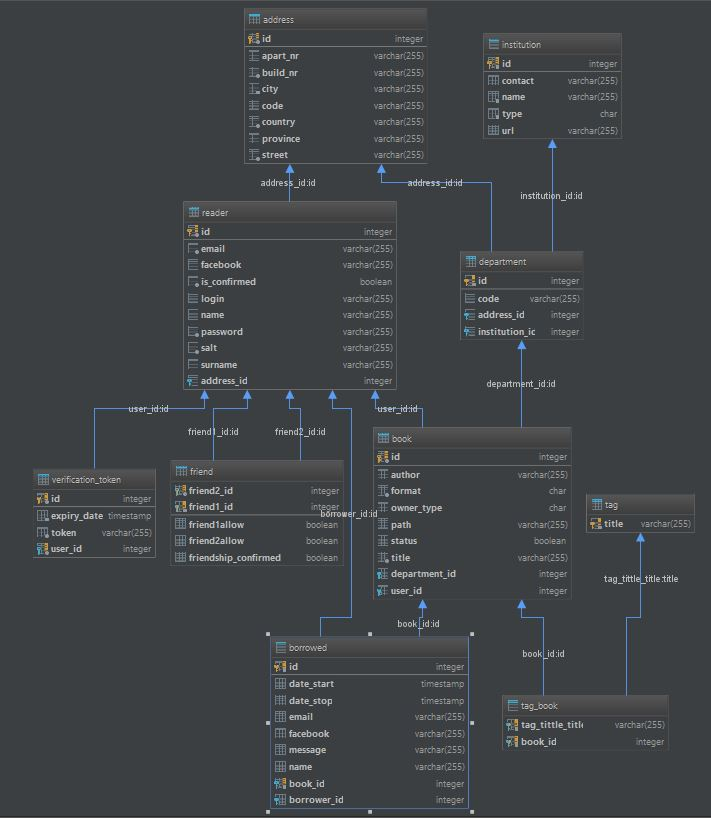
\includegraphics[width=1.\textwidth]{bookaDB.jpg}
			\end{figure}

\chapter{Opis techniczny}

	\section{Serwer aplikacji}
	
		\subsection{Podział aplikacji}

			W naszej aplikacji możemy wyszczególnić trzy podstawowe części - jest to baza danych, serwer aplikacji  i serwer WWW (nginx). Rozdzielenie dwóch ostatnich świadczy o tym, że nie jest to klasyczne podejście do aplikacji w architekturze MVC, jednak mimo to jest ona widoczna. W niniejszym podrozdziale skupimy się na podziale aplikacji z perspektywy serwera.
			
			\subsubsection{Kontroler}
			
Kontroler jest elementem, który przyjmuje dane od użytkownika, reaguje na jego poczynania. W naszej aplikacji jest to oczywiście kontroler REST'owy. Z serwera WWW wysyłane jest zapytanie na konkretny endpoint, który następnie odpowiada w sposób przez nas przewidziany (więcej o pkt. końcowych w punkcie 3.1.1). Na przykład w przypadku zapytania typu GET na adres <adres-ip>:8080/users	uprawniony użytkownik powinien otrzymać informacje o wszystkich użytkownikach w bazie w postaci listy json'ów. Poniżej przedstawiono implementację jednego z kontrolerów (najprostszego z nich).


\begin{lstlisting}[language=Java, breaklines]
@RestController
@RequestMapping(value = "/api/v1/tags")
public class TagController {

    @Autowired
    public TagService tagService;

    @RequestMapping(method = RequestMethod.GET)
    public Collection<Tag> getTags(){
        return tagService.getTags();
    }

    @RequestMapping(method = RequestMethod.POST)
    public ResponseEntity<Tag> addTag(@RequestBody Tag tag){
        try {
            return ResponseEntity.ok(tagService.addTag(tag));
        }
        catch (IllegalArgumentException e) {
            return new ResponseEntity<>(HttpStatus.CONFLICT);
        }
    }

    @RequestMapping(method = RequestMethod.DELETE)
    public ResponseEntity<Tag> deleteTag(@RequestBody String title) {
        Tag tag = tagService.getTagByTitle(title).orElse(null);

        if (tag == null)
        {
            return new ResponseEntity<>(HttpStatus.NOT_FOUND);
        }
        try {
            tagService.deleteTag(title);
        } catch (DataAccessException e) {
            return new ResponseEntity<>(HttpStatus.NOT_FOUND);
        }
        return new ResponseEntity<>(HttpStatus.OK);

    }
}
\end{lstlisting}
			
Adnotacje @RestController i @RequestMapping służą kolejno do oznaczenia, że dana klasa jest kontrolerem (typu REST'owego) oraz ścieżki od jakiej zaczynać się będą adresy wszystkich kontrolerów w tej klasie. @Autowired służy do podpięcia serwisu (jako, że serwis jest obiektem wyjątkowym, jedynym) - Spring Boot szuka tych adnotacji, tworzy i podpina do obiektu oznaczonego tą adnotacją. @RequestMapping użyte nad metodą wskazuje na dalsze rozwinięcie adresu i metodę HTTP jaką można się na ten adres odwoływać.

			
			\subsubsection{Serwis}
			
Serwis jest kolejnym poziomem abstrakcji odpowiedzialnym za obliczenia i pośredniczącym (jeżeli zachodzi taka potrzeba) pomiędzy kontrolerem a repozytorium. W warstwie serwisów są np. kodowane i dekodowane hasła, czy też ustalane linki do mapy na podstawie określonego adresu. Poniżej przedstawiono interfejs oraz implementację jednego z serwisów.			

\begin{lstlisting}[language=Java, breaklines]
@Service
public interface TagService {

    Collection<Tag> getTags();

    Optional<Tag> getTagByTitle(String title);

    Tag addTag(Tag tag);

    void deleteTag(String title);

}
\end{lstlisting}

Adnotacja @Service wskazuje, że powyższy kod dotyczy serwisu.

\begin{lstlisting}[language=Java, breaklines]
@Component
public class TagServiceImpl implements TagService{

    @Autowired
    private TagRepository tagRepository;

    @Override
    public Collection<Tag> getTags() {
        return StreamSupport.stream(tagRepository.findAll().spliterator(), false).
                collect(Collectors.toList());
    }

    @Override
    public Optional<Tag> getTagByTitle(String title) {
        return Optional.ofNullable(tagRepository.findOne(title));
    }

    @Override
    public Tag addTag(Tag tag)throws IllegalArgumentException {
        try {
            return tagRepository.save(tag);
        }
        catch (DataAccessException e) {
            throw new IllegalArgumentException(e);
        }
    }

    @Override
    public void deleteTag(String title) throws IllegalArgumentException {
        if (title == null)
            throw new IllegalArgumentException("Cannot delete tag with unspecified title");

        if (!tagRepository.exists(title))
            throw new IllegalArgumentException("Cannot delete tag that does not exist");

        try {
            tagRepository.delete(title);
        }
        catch (DataAccessException e) {
            throw new IllegalArgumentException(e);
        }
    }
}
\end{lstlisting}

Powyżej widzimy implementację wcześniej opisanego interfejsu. @Component sprawia, że spring automatycznie znajdzie tą klasę i stworzy niezbędny obiekt. W powyższym przykładzie widzimy odwołania do repozytorium (tagRepository), o którym w następnym punkcie.

			\subsubsection{Repozytorium}
			
			
Repozytorium jest pewnym typem klasy, który zapewnia komunikację z bazą danych. W naszej aplikacji korzystaliśmy z repozytorium CRUDowego (CRUD - create, read, update and delete - podstawowa metoda komunikacji z bazą danych) rozszerzonego o hibernate - framework'a ułatwiającego realizację dostępu do bazy danych w szczególnych przypadkach (hibernate pozwala na pisanie własnych, bardziej skomplikowanych zapytań). Uznaliśmy, że standard JPA jest nam nie potrzebny. Poniżej przedstawiono jedną z klas typu repozytorium - każda taka klasa pozwala na dostęp do jednego z typów obiektów (więcej o typach obiektów i o modelach w rozdziale poświęconym bazie danych).

\begin{lstlisting}[language=Java, breaklines]
public interface UserRepository extends CrudRepository<User, Integer> {

    User findByLogin(String login);

    User findByEmail(String email);

    @Query("SELECT u" +
            " FROM User u" +
            " WHERE UPPER(u.name) like UPPER(CONCAT('%',:any,'%')) " +
            " OR UPPER(u.surname) like UPPER(CONCAT('%',:any,'%')) " +
            " OR UPPER(u.login) like UPPER(CONCAT('%',:any,'%'))" +
            " OR UPPER(u.email) like UPPER(CONCAT('%',:any,'%'))")
    Collection<User> findByAny(@Param("any") String any);
}
\end{lstlisting}

Implementacja repozytorium jest bardzo prosta, a w najlepszym przypadku nie wymaga pisania ani jednej metody. CrudRepository posiada kilka wbudowanych zapytań (takich jak findOne(), czy delete()), które działają na podstawie klucza głównego obiektu (więcej w 3.3 i 4.3), jednak pozwala ono również na pisanie własnych zapytań poprzez odpowiednie nazywanie metod - np. findByLogin. Więcej informacji na ten temat można znaleźć pod następującym adresem \url{http://docs.spring.io/spring-data/jpa/docs/1.5.1.RELEASE/reference/html/jpa.repositories.html#jpa.query-methods.query-creation}. W przypadku bardziej skomplkowanych zapytań korzystaliśmy z adnotacji @Query (dostarczonej przez hibernate), która pozwala na pisanie zapytań w pseudo-sqlowym języku (HQL). Więcej informacji na stronie \url{https://docs.jboss.org/hibernate/orm/3.3/reference/en/html/queryhql.html}.
			
		\subsection{System kont użytkowników}
		
			\subsubsection{Logowanie i sesja}

			Dane wpisane przez użytkownika w celu zalogowania się są wysyłane na odpowiedni endpoint. W celu ich weryfikacji stworzyliśmy specjalny serwis odpowiedzialny za autoryzację:

\begin{lstlisting}[language=Java, breaklines]		
@Component
public class AuthorizationServiceImpl implements AuthorizationService {

    private final Map<UUID, Session> sessions = new HashMap<>();

    @Autowired
    public HashingService hashingService;

    @Autowired
    private UserService userService;

    @Override
    public Optional<Session> getSession(UUID token) {
        return Optional.of(sessions.compute
        		(token, (t, s) -> Optional.ofNullable(s).
                    filter(es -> es.getExpiration().isAfter(Instant.now())).
                    orElse(null)));
    }

    @Override
    public boolean invalidateSession(UUID token) {
        return sessions.remove(token) != null;
    }

    @Override
    public Optional<Session> authenticate(Credentials credentials) {
        val session = userService.getByLogin(credentials.getLogin()).
                filter(u -> u.getPassword().equals(Base64.getEncoder().
                        encodeToString(hashingService.hash(credentials.getPassword().
                        toCharArray(), Base64.getDecoder().decode(u.getSalt()))))).
                map(u -> new Session(u));

        session.ifPresent(s -> sessions.put(s.getToken(), s));

        return session;
    }
}	
\end{lstlisting}

Jak widać w powyższym fragmencie kodu, do tego serwisu został podpięty serwis odpowiedzialny za haszowanie - hasło jest przez niego kodowane (na podstawie 'soli' przypisanej do użytkownika) i porównywane z tym co znajduje się w bazie. Taka implementacja spełnia podstawowe wymagania dot. bezpieczeństwa. Kolejnym elementem na który warto zwrócić uwagę jest tablica asocjacyjna zawierająca pary wartości tokenu i sesji. W punkcie końcowym odpowiedzialnym za logowanie za każdym razem tworzona jest taka para, z której klucz wysyłany jest w ciasteczku do użytkownika. Pozwala to na utrzymywanie sesji i weryfikację użytkownika w innych punktach końcowych.
			
			\subsubsection{System pocztowy}
			
Kiedy użytkownik tworzy konto, jego dane pojawiają się w bazie danych (po uprzednim wygenerowaniu soli i zakodowaniu hasła). Jednak jest to użytkownik niepotwierdzony przez system (co oznaczamy za pomocą flagi isConfirmed). W celu potwierdzenia konta na adres użytkownika wysyłany jest email. Dzieje się to dzięki klasie EmailSender.

\begin{lstlisting}[language=Java, breaklines]
@Component
public class EmailSender {


    @Autowired
    private JavaMailSender javaMailSender;

    public EmailStatus sendPlainText(String to, String subject, String text) {
        return sendM(to, subject, text, false);
    }

    public EmailStatus sendHtml(String to, String subject, String htmlBody) {
        return sendM(to, subject, htmlBody, true);
    }

    private EmailStatus sendM(String to, String subject, String text, Boolean isHtml) {
        try {
            MimeMessage mail = javaMailSender.createMimeMessage();
            MimeMessageHelper helper = new MimeMessageHelper(mail, true);
            helper.setTo(to);
            helper.setSubject(subject);
            helper.setText(text, isHtml);
            javaMailSender.send(mail);

            return new EmailStatus(to, subject, text).success();
        } catch (Exception e) {
            return new EmailStatus(to, subject, text).error(e.getMessage());
        }
    }
}
\end{lstlisting}

Jak widać w powyższym fragmencie kodu klasa ta korzysta z kilku podstawowych klas wykorzystywanych do obsługi poczty (MimeMessage, MimeMessageHelper) jak i z gotowego serwisu javaMailSender, którego konfiguracje można znaleźć w pliku application.properties.

\begin{lstlisting}[language=Java, breaklines]
spring.mail.host=smtp.gmail.com
spring.mail.port=587
spring.mail.username=teambooka
spring.mail.password=TeamBookaTeamBooka
spring.mail.protocol=smtp
spring.mail.properties.mail.smtp.starttls.enable=true
spring.mail.default-encoding=UTF-8
\end{lstlisting}


Maile, które wysyłamy zawierają w sobie link odwołujący się do specjalnego endpointa, który w pasku zapytań zawiera specjalny token identyfikujący użytkownika. Tokeny są przechowywane w bazie danych. Poniżej przedstawiono klasę typu encji (więcej w rozdziale dot. bazy danych) dla tokenów.


\begin{lstlisting}[language=Java, breaklines]
@Entity
@Data
@Builder
@NoArgsConstructor
@AllArgsConstructor
public class VerificationToken {
    public static final int EXPIRATION = 60 * 24;

    @Id
    @GeneratedValue(strategy = GenerationType.IDENTITY)
    private Integer id;

    @Column(nullable = false)
    private String token;

    @OneToOne(optional = false)
    private User user;

    @Column(nullable = false)
    private Date expiryDate;

    public Date calculateExpiryDate(int expiryTimeInMinutes) {
        Calendar cal = Calendar.getInstance();
        cal.setTime(new Timestamp(cal.getTime().getTime()));
        cal.add(Calendar.MINUTE, expiryTimeInMinutes);
        return new Date(cal.getTime().getTime());
    }

}
\end{lstlisting}

	Żeby móc wysłać użytkownikowi hiper-link potrzebowaliśmy jeszcze czegoś co pozwalałoby nam modyfikować kod HTML'a na podstawie zmiennych z aplikacji. W tym celu użyliśmy silnika thymeleaf. Poniżej przedstawiono przygotowanego kod wykorzystujący wspomniany silnik i template'a

\begin{lstlisting}[language=Java, breaklines]	
@Component
public class EmailHtmlSender {

    @Autowired
    private EmailSender emailSender;

    @Autowired
    private TemplateEngine templateEngine;

    public EmailStatus send(String to, String subject, String templateName, Context context) {
        String body = templateEngine.process(templateName, context);
        return emailSender.sendHtml(to, subject, body);
    }
}
\end{lstlisting}

\begin{lstlisting}[language=HTML, breaklines]
<!DOCTYPE html>
<html xmlns:th="http://www.thymeleaf.org">
<head>
    <title th:remove="all">Confirmation</title>
    <meta http-equiv="Content-Type" content="text/html; charset=UTF-8"/>
</head>
<body>
Your account was successfully created. Please click the link below<br>
to confirm your email address and activate your account:
<p>
    <a th:text=${link} th:href="@{'http://' + ${link}}">"${link}"</a>
</p>
<p>
    --<br>
    Questions? Comments? We don't care
</p>
</body>
</html>
\end{lstlisting}

	

		\subsection{Przeszukiwanie zasobów bibliotecznych}
		
			\subsubsection{Formułowanie zapytań do zasobów bibliotecznych}
		
				Konstrukcja podstawowych zapytań do zasobów bibliotecznych jest stosunkowo prosta. Używany jest do tego język poleceń CCL (Common Command Language), umieszczany w linku wraz z komendą wyszukania książek. Przykładowo:
				
				\begin{center}
					$ ((wau=George$ $or$ $Martin) and (wti=Pieśń?)) $\\
				\end{center}

			\subsubsection{Pola dopuszczalne w zapytaniu}
			
				Poniżej lista możliwych zmiennych poprzez które możemy się odwoływać bezpośrednio do bazy danych.
				
				\begin{itemize}
					\item TIT - Titles - Tytuły
					\item AUT - Authors - Autorzy
					\item IMP - Imprint - Wydano
					\item SUB - Subjects - Hasła przedmiotowe
					\item SRS - Series - Serie
					\item LOC - Location - Sygnatura
				\end{itemize}
				
				Wykorzystanie powyższych pól wymaga większej precyzji w umieszczanych tam danych. Lepszym rozwiązaniem wydają się zmienne typu słowa, odpowiadają one zawartości pół uzupełnianych ręcznie przez użytkownika na stronie co sugeruje mniej rygorystyczne zasady ich uzupełniania.
				
				\begin{itemize}
					\item WRD - Words - Słowa
					\item WTI - Words in title field - Słowa z pola tytułu
					\item WAU - Words in author field - Słowa z pola autora
					\item WPE - Words in personal author field - Słowa z pola autora indywidualnego
					\item WCO - Words in corporate author field - Słowa z pola autora korporatywnego
					\item WME - Words in meeting field - Słowa z pola imprez
					\item WUT - Words in uniform title field - Słowa z pola tytułu ujednoliconego
					\item WPL - Words in place field - Słowa z pola miejsca wydania
					\item WPU - Words in publisher field - Słowa z pola wydawcy
					\item WSU - Words in subject field - Słowa z pola haseł przedmiotowych (odpowiednik tagów)
					\item WSM - Words in MeSH subjects - Słowa z haseł MeSH
					\item WST - Words in status - Słowa w statusie
					\item WGA - Words in geographical area - Słowa z haseł geograficznych
					\item WYR - Year of publication - Rok publikacji 
				\end{itemize}
		
			\subsubsection{Operatory logiczne i formatowanie zapytań}
			
				Jak widać zapytanie posiada operatory logiczne do składania jego treści. Każde z nich może być zastąpione odpowiednikiem podanym poniżej.
				
				\begin{itemize}
					\item AND = +/\&
					\item OR = |
					\item NOT = \textasciitilde
				\end{itemize}
				
				Oprócz powyższych podstawowych zasad tworzenia zapytań są jeszcze dodatkowe:
				
				Znak ? lub * (gwiazdka), mogą być stosowane w słowie, ale nie mogą występować częściej niż raz w zapytaniu.
				
				Symbol \# może służyć do wyszukiwania różnych wersji pisowni, gdy jedna wersja słowa posiada jeden znak więcej niż druga. Na przykład, colo\#r spowoduje wyszukanie zarówno słowa color jak i colour; a arch\#eology spowoduje wyszukanie zarówno słowa archaeology jak i archeology.
				
				Znak ! może służyć do wyszukiwania różnych wersji pisowni, w przypadkach gdy pisownia może różnić się jednym znakiem. Na przykład, wom!n spowoduje wyszukanie zarówno słowa woman jak i women.
				
				Znak ! poprzedzający numer, można umieszczać pomiędzy słowami, aby określić maksymalny odstęp pomiędzy słowami, z zachowaniem kolejności występowania słów. W tym przypadku, ballads !3 england spowoduje wyszukanie Ballads of England i Ballads of Merry Olde England ale nie England and Her Ballads.
				
				Symbol \% poprzedzający numer, można umieszczać pomiędzy słowami, aby określić maksymalny odstęp pomiędzy słowami, niezależnie od ich kolejności. na przykład, england \%3 ballads spowoduje wyszukiwanie Ballads of England , Ballads of Merry Olde England i England and Her Ballads.
				
				Pomiędzy słowami mogą być umieszczane symbole -> (myślnik i znak większości). Oznacza to, że chcemy wyszukać rekordy, które zawierają słowa od pierwszego słowa (włącznie) aż do drugiego. To wyszukiwanie jest szczególnie przydatne do ograniczenia zestawu rekordów ze względu na rok wydania. Np: 1993 -> 1996.
				
			\subsubsection{Przeszukiwanie konkretnych bibliotek}
				
				Możliwy jest też wybór biblioteki w której szukamy książki, polega to na dodaniu na końcu zapytania formuły $\&local\_base=\underline{nr}$, gdzie  $\underline{nr}$ oznacza numer szukanej biblioteki w systemie. Poniżej tabela oddziałów i ich numery systemowe.
				
				\begin{longtable}{|p{2cm}|p{6cm}|}
					\caption{Oddziały biblioteki miejskiej} \label{lib_0} \\ \hline
					Numer Filii & Lokacja  \\ \hline
					01 & ul. Sztabowa 98 (ALEPH) \\ \hline
					02 & ul. Eluarda 51-55 (ALEPH)  \\ \hline
					03 & ul. Morelowskiego 43 (ALEPH)  \\ \hline
					04 & ul. Wieczysta 105 (ALEPH)  \\ \hline
					05 & ul. Namysłowska 8 - Grafit (ALEPH)  \\ \hline
					06 & ul. Lwowska 21 (ALEPH)  \\ \hline
					07 & ul. Suwalska 3 (ALEPH)  \\ \hline
					08 & ul. Głogowska 9-11  \\ \hline
					09 & ul. Wielkopolska 16  \\ \hline
					10 & ul. Jelenia 7 (ALEPH)  \\ \hline
					11 & ul. Krzywoustego 286 - Fama (ALEPH)  \\ \hline
					15 & ul. Rękodzielnicza 1  \\ \hline
					16 & ul. Kolista 17 (ALEPH)  \\ \hline
					17 & ul. Gałczyńskiego 8 (ALEPH)  \\ \hline
					18 & ul. Grabiszyńska 236a (ALEPH)  \\ \hline
					20 & ul. Majakowskiego 34/1a \\ \hline
					22 & ul. Chociebuska 8-10 (ALEPH) \\ \hline
					23 & bul. Ikara 29-31 (ALEPH) \\ \hline
					26 & ul. Olszewskiego 85a (ALEPH)  \\ \hline
					27 & ul. Łokietka 13 (ALEPH) \\ \hline
					29 & ul. Reja 1-3 (ALEPH) \\ \hline
					31 & ul. Strachocińska 88 \\ \hline
					32 & ul. 9 Maja 26 \\ \hline
					37 & ul. Sempołowskiej 54a (ALEPH) \\ \hline
					40 & ul. Przybyszewskiego 59 (ALEPH) \\ \hline
					41 & ul. Sołtysowicka 48 \\ \hline
					42 & ul. Serbska 5a (ALEPH) \\ \hline
					44 & ul. Powstańców Śl. 210 (ALEPH) \\ \hline
					45 & ul. Traugutta 82 (ALEPH) \\ \hline
					46 & ul. Tarnogórska 1 (ALEPH) \\ \hline
					47 & ul. Polna 4 (ALEPH) \\ \hline
					53 & ul. Hercena 13 \\ \hline
					54 & ul. Jesienna 22 (ALEPH) \\ \hline
					55 & ul. Zielińskiego 2 (ALEPH) \\ \hline
					57 & ul. Szewska 78 (ALEPH) \\ \hline
					58 & pl. Teatralny 5 - Mediateka (ALEPH) \\ \hline
					64 & ul. Osobowicka 127 \\ \hline
					69 & ul. Wróblewskiego 1-5 (ZOO)\\ \hline
					70 & ul. Wittiga 10 (Biblioteka Parafialna)\\ \hline
				\end{longtable}
			
			\subsubsection{Filtrowanie otrzymywanych wyników}
				
				Możliwe sa również opcje filtrowania ustawiane już w zapytaniu do serwera. Zapytania takie są kolejnym członem podstawowego zapytnia CCL. Poniżej możliwe elementy takiego zapytania oraz dopuszczalne parametry. 
				
				\begin{itemize}
					\item WFT - szukany format 
					\begin{itemize}
						\item BK - książki 
						\item SE - czasopismo 
						\item MU - aubiobook 
						\item MP - mapa 
						\item CF - ebook
						\item VM - film 
						\item PD - pomoc dydaktyczna 
					\end{itemize}
					\item WLN - wybór języka poszukiwanego dzieła
					\begin{itemize}
						\item POL - polski
						\item ENG - angielski
						\item FRE - francuski
						\item GER - niemiecki
					\end{itemize}
				\end{itemize}
			
			\subsubsection{Zaimplementowane mechanizmy formułowania zapytań}
				
				Najprostszym sposobem jest utworzenie zapytania składającego się jedynie z wypełnionego pola WRD, gdzie można umieścić wszystkie możliwe elementy zapytania, jednak zrezygnowaliśmy z tego na rzecz bardziej szczegółowego zapytania składanego z pół odpowiednich danych, kolejno WAU jako pole z szukanym autorem, WTI jako pole z tytułem książki oraz numer systemowy oddziału biblioteki. Oczywiście jeśli któryś z wymienionych elementów jest nieobecny w zapytaniu, przychodzącym do serwera, zostaje on również pominięty przy tworzeniu zapytania.
				
				Poniżej znajduje się przykład całego złożonego zapytania z podkreślonym edytowanym przez nas fragmentem.
				
				\begin{center}
					$ https://katalog.biblioteka.wroc.pl/F?func=find-c\&ccl\_term=\underline{((WAU=George OR Martin)AND(WTI=Pieśń?))and(WFT=(BK))\&local\_base=31} $
				\end{center}
			
			\subsubsection{Pobieranie danych z systemu bibliotecznego}
			
			Z powodu braku możliwości uzyskania bezpośredniego dostępu do bazy danych biblioteki publicznej w Wrocławiu, dane musieliśmy uzyskiwać w inny sposób. Wykorzystaliśmy powyższe metodykę zapytań oraz bibliotekę Jsoup udało się nam tego dokonać. Należy tutaj wytłumaczyć iż Jsoup posiada API do wydobywania i manipulowania danymi uzyskiwanymi z plików HTML.
			
			Przy każdym zapytaniu na nasz serwer, tworzymy zapytanie do sytemu bibliotecznego zgodnie z wcześniej opisaną formuła. Następnie schodzimy pod uzyskane adresu z poziomu serwera, który również otrzymuje zwrotny HTML ze stroną zawierającą odpowiedź biblioteki na wysłane zapytanie. Tutaj otrzymana strona jest parsowana w odpowiedni sposób, a uzyskane dane dostosowywane do modelu książki opisanego w naszym systemie i zwracane do strony z której przyszło zapytanie.
		
	\section{Aplikacja internetowa}
	
		%inne, jakiś tam podział na kontolery itp.
	
		\subsection{Kolejka komunikatów}
		
		\subsection{Google Drive}
	
	\section{Baza danych}
	
		Jak znaczna część konfiguracji tak i zmienne potrzebne do zalogowania się do bazy danych znajdują się w pliku "application.properties":

		\begin{itemize}
			\item spring.datasource.url - zmienna przyjmująca adres bazy danych. Domyślną wartość stanowi "jdbc:postgresql://localhost:5432/BookaDB"
			\item spring.datasource.username - nazwa użytkownika bazy danych. Domyślnie jest to "postgres"
			\item spring.datasource.password - hasło do bazy danych. Domyślnie jest to "postgres"
		\end{itemize}

		Każdy obiekt typu encji (więcej w poprzednim rozdziale) został stworzony wg. powtarzalnego schematu, który zostanie objaśniony na podstawie poniższego fragmentu kodu.

		\begin{lstlisting}[language=Java, breaklines]
@Entity
@Table(name="Reader")
@Data
@Builder
@NoArgsConstructor
@AllArgsConstructor
public class User implements Serializable {

    @Id
    @GeneratedValue(strategy = GenerationType.IDENTITY)
    private Integer id;

    private String login;

    @Column(nullable = false)
    private String password;

    @Column(nullable = false)
    private String email;

    @Column(nullable = false)
    private String salt;

    @Column(nullable = false)
    private Boolean isConfirmed;

    @OneToOne
    private Address address;
    private String name;
    private String surname;
    private String facebook;
}
		\end{lstlisting}

		Każdy klasa implementująca obiekty typu encji musi zaczynać się od adnotacji "@Entity". Adnotacja @Table daje dostęp do kontroli tego, w jaki sposób zostanie stworzona tabela reprezentująca daną klasę. Na przykładzie widać w jaki sposób można nadać nazwę tabeli (domyślna wartość jest równa nazwie klasy). Cztery kolejne adnotacje pochodzą z narzędzia "lombok" pozwalającego na automatyczne wygenerowanie standardowych metod (takich jak np gettery i settery). Przejdźmy do ciała klasy - każde pole reprezentuje kolejną kolumnę, a adnotacje nad polami pozwalają sterować tym w jaki sposób dane pole zostanie odwzorowane w bazie danych. Adnotacją "@Id" oznacza się klucz główny, @GeneratedValue mówi o tym, że wartość powinna być wygenerowana automatycznie, @Column pozwala na sterowanie parametrami pól, @OneToOne wskazuje na typ relacji pomiędzy dwoma obiektami (adnotacja musi znajdować się nad zdefiniowanym przez nas obiektem). Istnieje wiele innych, ciekawych możliwości pozwalających budować modele obiektów, jednak wymienienie ich wszystkich niej jest celem tej dokumentacji. Należy jednak wspomnieć o jeszcze jednym ważnym elemencie jakim jest adnotacja @Embededkey. Pozwala ona na tworzenie kluczy złożonych i stosowana jest analogicznie do @Id z tym że nad specjalnie stworzonym przez nas polu typu id. Poniżej przedstawiono przykład.


		\begin{lstlisting}[language=Java, breaklines]
@Entity
@Data
@Builder
@NoArgsConstructor
@AllArgsConstructor
public class Friend implements Serializable{

    @EmbeddedId
    private FriendId friendId;

    private Boolean friend1Allow;
    private Boolean friend2Allow;

    private Boolean friendshipConfirmed;

}
		\end{lstlisting}

		\begin{lstlisting}[language=Java, breaklines]
@Embeddable
@Data
@Builder
@NoArgsConstructor
@AllArgsConstructor
public class FriendId implements Serializable{

    @ManyToOne(optional = false)
    @OnDelete(action = OnDeleteAction.CASCADE)
    private User friend1;

    @ManyToOne(optional = false)
    @OnDelete(action = OnDeleteAction.CASCADE)
    private User friend2;
}
		\end{lstlisting}


\chapter{Opis funkcjonalny}

	\section{Instalacja i konfiguracja systemu}
	
	\section{Opis funkcjonalności}


\chapter{Spis tabel i obrazów}


\begingroup
\let\clearpage\relax
\listoffigures
\listoftables
\endgroup



\end{document}
